\documentclass[a4paper,10pt]{report}
\usepackage[utf8]{inputenc}
\usepackage{hyperref}
\usepackage{svg}
\usepackage{graphicx}
\usepackage{float}
\usepackage{parskip}
\usepackage[frenchb]{babel}
\usepackage[T1]{fontenc}
\usepackage[nonumberlist]{glossaries}
\usepackage[inline]{asymptote}

\makeglossaries
% entrées du lexique
\newglossaryentry{training}
{
  name={entraînement},
	description={Lorem ipsum dolor sit amet}
}
\newglossaryentry{carvec}
{
  name={vecteur de caractéristiques},
	description={En reconnaissance de formes, un vecteur de caractéristiques est une représentation numérique de
	propriétés visuelles d'un objet. Il peut par exemple être constitué de la quantité de lignes présentes dans
	l'image selon leur orientation, chaque orientation constituant une dimension du vecteur. Ces représentations
	permettent d'effectuer des traitements statistiques, comme des régressions linéaires}
}

\newglossaryentry{CNN}
{
  name={CNN},
	description={Lorem ipsum dolor sit amet}
}
\newglossaryentry{MLNN}
{
  name={MLNN},
	description={En reconnaissance de formes, un vecteur de caractéristiques est une représentation numérique de
	propriétés visuelles d'un objet. Il peut par exemple être constitué de la quantité de lignes présentes dans
	l'image selon leur orientation, chaque orientation constituant une dimension du vecteur. Ces représentations
	permettent d'effectuer des traitements statistiques, comme des régressions linéaires}
}

%opening
\title{}
\author{}
\setlength{\parindent}{15pt}

\begin{document}

\maketitle

\chapter{Deep Learning}

\section{Machine Learning}

\subsection{Principes généraux}

Le Machine Learning, également connu sous le terme d'apprentissage automatique, est un sous-domaine de l'intelligence artificielle, ayant vu le jour dans
les années 1950\cite{Bib_Marr}\cite{Bib_McCar}
Son champ d'application est aujourd'hui très vaste, et sa principale limite réside en la quantité d'informations exploitables, disponible au sein d'un domaine donné.


L'accroissement de la collecte, du stockage et de la mise à disposition des données que nous connaissons depuis quelques années a permit l'essor de ces algorithmes et leur transposition à de nombreux problèmes :

\begin{itemize}
  \item la classification de contenu audio-visuel au sens large, allant de l'image au sujet d'un texte ou d'une revue
  \item le filtrage de contenus, tels que les spams ou les intrusions sur les systèmes d'informations
  \item le tri et la sélection d'informations les plus pertinentes à délivrer via la publicité ou les flux de contenus des médias sociaux
  \item l'analyse de sentiments
\end{itemize}

Plus précisément, ce concept recouvre les systèmes constitués de paramètres réglables, typiquement vus sous la forme de
valeurs vectorielles, en vue de fournir la sortie attendue pour une série de valeurs données en entrée. En outre, ce type d'apprentissage se distingue
par sa capacité à ajuster ses paramètres de manière autonome, en se basant sur l'expérience des données précédemment traîtées.

Dans ce qui va suivre, cette technique sera abordée à la lumière des problèmes de reconnaissance de formes, les entrées dont il sera alors question étant des images ou des vidéos.

\subsection{Systèmes de reconnaissance de formes}

L'architecture d'un système de reconnaissance de formes comprend deux éléments principaux :

\begin{itemize}
  \item un extracteur des caractéristiques de l'entrée
  \item un classifieur qui donne le résultat en sortie, associant généralement l'entrée à une classe
\end{itemize}



Dans les années 50, les premiers modèles de reconnaissance étaient constitués d'un extracteur de caractéristiques "fait-main", peu modulaire et fastidieux à implémenter\cite{Bib_LeCun}.
C'est lui qui est chargé de traduire l'image, ou partie de l'image, en une représentation vectorielle des motifs qu'elle contient.
\par
Dans un deuxième temps, le classifieur détermine la classe résultante selon une somme pondérée des composantes du \gls{carvec}.
Une valeur seuil est fixée de telle sorte à ce que la sortie soit activée ou non en fonction du calcul précédent.
Lorsque des erreurs sont repérées en sortie, cet algorithme va réajuster ses paramètres internes en vue d'améliorer les réponses suivantes. On parle alors d'entraînement.
\par
Dans le cadre d'une classification dite linéaire, ces réglages s'effectuent sur la valeur des poids associés aux caractéristiques.
L'enjeu du classifieur est de réduire la différence entre les résultats attendus $\hat{y}$, et effectifs $y$.
La phase d'entraînement revient à minimiser une fonction objectif\footnote{Dans le framework Caffe, une telle fonction est désignée sous le nom de loss function.}, en modulant les pondérations ($\theta$).
D'un point de vue mathématique, la fonction objectif peut différer en fonction de l'approche adoptée. On la trouvera par exemple sous forme de moindres carrés de résidus\cite{Bib_WikiLS} :

\begin{center} $ E = J({\theta}) =  \sum\limits_{i=1}^{n} (y_{i} - \hat{y}_{i} )^2 $ \end{center}

ou d'erreur quadratique moyenne\cite{Bib_WikiMSE} :

\begin{center} $ E = J({\theta}) =  \frac{1}{n}\sum\limits_{i=1}^{n} (y_{i} - \hat{y}_{i})^2 $ \end{center}

Un tel comportement correspond à un apprentissage supervisé, où la réponse correcte est connue, permettant à la machine de s'améliorer. Une fois cette phase achevée, le système est théoriquement apte à
classifier avec exactitude de nouvelles entrées, jusqu'alors inconnues : c'est la généralisation.
\par
D'autre part, comme représenté figure~\ref{fig:c1p1s2}, l'approche par apprentissage profond vise à étendre les capacités d'entraînement et de généralisation à l'ensemble de la chaîne de reconnaissance de formes.
Notre étude se base sur ce dernier modèle, où l'extracteur de caractéristiques, aussi appelé noyau, peut être entraîné.

\begin{figure}[H]
    \centering
    \makebox[\textwidth]{\includesvg[width=.6\paperwidth]{c1p1s2_schema}}
    \caption{Différentes approches de la reconnaissance de formes}
    \label{fig:c1p1s2}
\end{figure}

\section{Réseaux de neurones}

\subsection{Neurone artificiel}

A la base des réseaux de neurones se trouve le concept de neurone formel représenté sur la figure\ref{fig:c1p2s1}.
\par
\begin{figure}[H]
    \centering
    \makebox[\textwidth]{\includesvg[width=.4\paperwidth]{c1p2s1_neuron}}
    \caption{Schéma d'un neurone formel}
    \label{fig:c1p2s1}
\end{figure}

Nous retrouvons les entrées $x_{i}$ qui correspondent dans notre cas aux i composantes du vecteur de caractéristiques donné par l'extracteur.
Ces entrées sont ensuite sommées avec leur poids $\theta_{i}$ (ou coefficient synaptique) respectif, ainsi qu'un coefficient $\theta_{0}$ appelé biais.
Le résultat pondéré est ensuite transmis à une fonction d'activation non linéaire\cite{Bib_WikiAN}. Celle-ci activera la synapse suivante (ici, la sortie), si son résultat dépasse un seuil donné.
\par
En pratique, plusieurs fonctions d'activation peuvent être choisies au regard de leurs caractéristiques.
Parmi les plus utilisées, on peut citer les fonctions sigmoïdes et tangentes hyperboliques. Leur efficacité tient notamment du fait qu'elles soient indéfiniement et rapidement dérivables et non polynômiales.
\par
Admettons que ce système contienne des entrées sous forme de vecteurs à $n$ dimensions, étiquettés selon les classes $C_{0}$ et $C_{1}$. Le but de l'entraînement sera d'obtenir en sortie : \\

\begin{center}

$\left\{
\begin{array}{ll}
 y=0,$ si $ x\in C_{0} \\
 y=1,$ si $ x\in C_{1}
\end{array}
\right.\ , \forall x
$

\end{center}
sachant que,
\begin{center}
$ y = \phi( \sum\limits_{i=1}^{n}(x_{i}\theta_{i}) + \theta_{0} ),$ avec $\phi$ fonction d'activation
\end{center}

le problème revient à trouver la valeur optimale du vecteur $\theta$, permettant de séparer linéairement les classes.
La figure\ref{fig:c1p2s1_2} illustre ce concept dans le cadre d'une classification d'éléments à deux dimensions, distribués entre deux classes.

\begin{figure}[H]
    \centering
    \makebox[\textwidth]{\includesvg[width=.4\paperwidth]{c1p2s1_points}}
    \caption{Classes linéairement séparables}
    \label{fig:c1p2s1_2}
\end{figure}

\subsection{Réseau multicouches}

Les problèmes traditionnels de classification nécessitent des modèles plus élaborés, car ils sont souvent insolubles à l'aide de simples régressions linéaires. On dit que l'ensemble des éléments constituant nos classes
sont non linéairement séparables (les résultats de la fonction XOR par exemple). On organise alors les neurones formels en successions de couches, ce qui permettra de diviser le plan en $n$ sous-ensembles, avec $n >2$.
On appelle typiquement \textit{couche d'entrée} la première couche du réseau, \textit{couches cachées} les couches internes au réseau et \textit{couche de sortie} la dernière couche.
Issue du site de tensorflow\cite{Bib_PlaygroundTF} (la librairie de calcul de machine learning développée par Google\cite{Bib_TenFlo}), la capture d'écran\ref{fig:c1p2s2} illustre les jeux de données pour lesquelles les régressions linéaires s'avèrent inefficaces.

\begin{figure}[H]
    \centering
    \makebox[\textwidth]{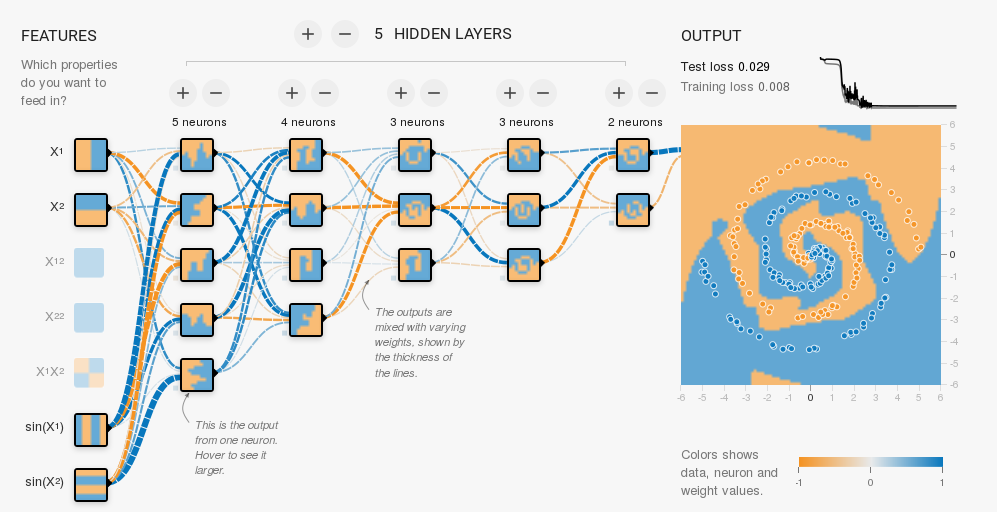
\includegraphics[width=.6\paperwidth]{c1p2s2_tensorflow}}
    \caption{Simulation tensorflow}
    \label{fig:c1p2s2}
\end{figure}


Dans cette configuration, les interactions entre les différents neurones, et les différentes couches, correspondent à ce qui a été décrit précédemment. L'information se propage `en avant` (\textit{forward propagation} ou \textit{feed forward}).
\par
Pour ajuster les poids synaptiques lors de l'entraînement, chaque neurone formel calcule l'erreur locale dûe à la modification d'un poids (c'est l'équivalent de l'erreur globale présentée section 1.1.2, limitée à deux neurones).
La méthode de descente de gradient stochastique\cite{Bib_WikiSGD} va permettre d'estimer l'incrément ou le décrément d'erreur correspondant à la modification du poids en question. Cela consiste à dériver partiellement la fonction d'erreur par le poids local.

\begin{center}
$\Delta \theta_{i,j} = -\alpha \dfrac{\partial E} {\partial \theta_{i,j}} $ , avec
$\left\{
\begin{array}{ll}
 \Delta \theta_{i,j} $, variation de $\theta$ entre les neurones $i$ et $j$ $\\
 \alpha $, le pas d'apprentissage $\\
 E $, fonction d'erreur $
\end{array}
\right.
$
\end{center}

Notons qu'une valeur de $\alpha$ élevée augmente le risque de dépasser le minimum recherché, tandis qu'une valeur trop petite va rallonger la phase d'entraînement.
\par
Les difficultés à calculer cette dérivée à n'importe quel niveau du réseau mènent à utiliser la technique de la rétropopagation\cite{Bib_WikiBP} (\textit{backpropagation}). L'erreur est alors estimée par la couche de sortie (qui a connaissance du résultat)
, puis relayée aux niveaux inférieurs, simplifiant ainsi leur descente de gradient respective.

\section{Réseaux convolutifs}

\subsection{Autres}
deep learning : connu depuis 1980 mais répandu depuis 2012
perceptron
capacité de généralisation : faculté d'un système à produire des résultats corrects sur des entrées inconnues, après un phase d'entraînement
rétropopagation : depuis les années 80
gardient : incrément ou décrément calculable de l'erreur correspondant à la modification des poids $\theta$ lors de la phase d'entraînement



% ajoute le lexique
\setglossarystyle{altlist}
\printglossaries


\begin{thebibliography}{9}

\bibitem{Bib_Marr}
Bernard Marr,
\emph{A short history of machine learning},
Forbes.com, 19 février 2016,
\url{http://www.forbes.com/sites/bernardmarr/2016/02/19/a-short-history-of-machine-learning-every-manager-should-read/fdc5dfd323ff}.

\bibitem{Bib_McCar}
John McCarthy,
\emph{Arthur Samuel: Pioneer in Machine Learning },
Stanford University, Stanford, California, USA -
Stanford Computer Science,
\url{http://infolab.stanford.edu/pub/voy/museum/samuel.html}.

\bibitem{Bib_LeCun}
Yann LeCun,
\emph{Recherches sur l'intelligence artificielle},
Collège de France, France,
7p,
\url{https://www.college-de-france.fr/site/yann-lecun/Recherches-sur-l-intelligence-artificielle.htm}.

\bibitem{Bib_WikiLS}
Wikipedia, \emph{Least squares},
\url{https://en.wikipedia.org/wiki/Least_squares}.

\bibitem{Bib_WikiMSE}
Wikipedia,
\emph{Mean squared error},
\url{https://en.wikipedia.org/wiki/Mean_squared_error}.

\bibitem{Bib_WikiAN}
Wikipedia,
\emph{Artificial neuron},
\url{https://en.wikipedia.org/wiki/Artificial_neuron}.

\bibitem{Bib_PlaygroundTF}
Playgroung TensorFlow,
\emph{Tinker with a neural network in your browser},
\url{http://playground.tensorflow.org}.

\bibitem{Bib_TenFlo}
TensorFlow,
\emph{Open source software library for machine intelligence},
\url{https://www.tensorflow.org/}.

\bibitem{Bib_WikiSGD}
Wikipedia,
\emph{Stochatstic gradient descent},
\url{https://en.wikipedia.org/wiki/Stochastic_gradient_descent}.

\bibitem{Bib_WikiBP}
Wikipedia,
\emph{Backpropagation},
\url{https://en.wikipedia.org/wiki/Backpropagation}.

\bibitem{Bib_ZeFer}
Matthew D Zeiler, Rob Fergus,
28 Nov 2013,
Cornell University Library, Ithaca, NY, USA -
Computer vision and pattern recognition,
11p
\emph{Visualizing and Understanding Convolutional Networks, v3},
\url{https://arxiv.org/abs/1311.2901}.

\end{thebibliography}

\end{document}
